% $Header: /cvsroot/latex-beamer/latex-beamer/examples/beamerexample5.tex,v 1.22 2004/10/08 14:02:33 tantau Exp $

\documentclass[11pt]{beamer}
\date{\today}

\usetheme{Darmstadt}

\usepackage{times}
\usefonttheme{structurebold}

%\usepackage[english]{babel}
\usepackage[portuges]{babel}
\usepackage{pgf,pgfarrows,pgfnodes,pgfautomata,pgfheaps}
\usepackage{amsmath,amssymb}
\usepackage[latin1]{inputenc}
\usepackage{graphicx}

\setbeamercovered{dynamic}

\newcommand{\Lang}[1]{\operatorname{\text{\textsc{#1}}}}

\newcommand{\Class}[1]{\operatorname{\mathchoice
  {\text{\sf \small #1}}
  {\text{\sf \small #1}}
  {\text{\sf #1}}
  {\text{\sf #1}}}}

\newcommand{\NumSAT}      {\text{\small\#SAT}}
\newcommand{\NumA}        {\#_{\!A}}

\newcommand{\barA}        {\,\bar{\!A}}

\newcommand{\Nat}{\mathbb{N}}
\newcommand{\Set}[1]{\{#1\}}

\pgfdeclaremask{tu}{beamer-tu-logo-mask}
\pgfdeclaremask{computer}{beamer-computer-mask}
\pgfdeclareimage[interpolate=true,mask=computer,height=2cm]{computerimage}{beamer-computer}
\pgfdeclareimage[interpolate=true,mask=computer,height=2cm]{computerworkingimage}{beamer-computerred}
\pgfdeclareimage[mask=tu,height=.5cm]{logo}{logounesp}

\logo{\pgfuseimage{logo}}

\title{Relaes de Maxwell}
\author{Ney Lemke}
\institute[IBB-UNESP]{%
    Biofísica e Farmacologia}
\date{ 2011}                                

\colorlet{redshaded}{red!25!bg}
\colorlet{shaded}{black!25!bg}
\colorlet{shadedshaded}{black!10!bg}
\colorlet{blackshaded}{black!40!bg}

\colorlet{darkred}{red!80!black}
\colorlet{darkblue}{blue!80!black}
\colorlet{darkgreen}{green!80!black}

\def\radius{0.96cm}
\def\innerradius{0.85cm}

\def\softness{0.4}
\definecolor{softred}{rgb}{1,\softness,\softness}
\definecolor{softgreen}{rgb}{\softness,1,\softness}
\definecolor{softblue}{rgb}{\softness,\softness,1}

\definecolor{softrg}{rgb}{1,1,\softness}
\definecolor{softrb}{rgb}{1,\softness,1}
\definecolor{softgb}{rgb}{\softness,1,1}

\AtBeginSection[]{\frame{\frametitle{Outline}\tableofcontents[current]}}

\begin{document}

\frame{\titlepage}

%\section*{Outline}

\part{Parte I}
\frame{\frametitle{Outline}\tableofcontents[part=1]}

\section{Foras Generalizadas}

\frame{\frametitle{Foras generalizadas}
Foras Generalizadas so grandezas que controlam uma
determinada grandeza extensiva. Um exemplo trivial
 $-p$ que controla o Volume. Mas existem muitas outras possibilidades:
 \begin{itemize}
 \item $[f,l]$ fora e comprimento
 \item $[\gamma, a]$ tenso superficial e rea
 \item $[\psi,q]$  potencial e carga
 \item $[B,I]$ campo magntico e momento magntico
 \end{itemize}

No caso geral denotamos por:

$$P_j= \left( \frac{\partial U}{\partial X_j}\right)_{S,V,N,X_{i,i\neq j}}$$

}


\frame{\frametitle{Tenso Superficial}

$$dU=TdS-pdV+\sum_{j=1}^M\mu_j dN_j +\gamma da$$

Experimentalmente conseguimos controlar as variveis:$T,p,N$ e $\gamma$.
Qual o potencial termodinmico de interesse neste caso. Ou seja queremos
que esta funo atinja um extremo no equilbrio.

Note que no equilbrio e $p$, $N$ e $T$ constantes
$$d(U-TS+pV-\gamma a)=-SdT +Vdp+\sum_{j=1}^M\mu_j dN_j-ad\gamma=0$$
$$d(G-\gamma a)=0$$

}

\frame{\frametitle{rea}
Qual funo  a mais relevante quando a rea  conservada?

$$dU=TdS-pdV+\sum_{j=1}^M\mu_j dN_j +\gamma da$$

$$d(U-TS+pV)=-SdT +Vdp+\sum_{j=1}^M\mu_j dN_j+\gamma da=$$

$$dG$$
}

\section{Relaes de Maxwell}

\frame{\frametitle{Derivadas Parciais}
As relaes de Maxwell esto baseadas na seguinte propriedade
das derivadas parciais:

$$\left(\frac{\partial^2 U}{\partial V\partial S}\right)=
  \left(\frac{\partial^2 U}{\partial S\partial V}\right)$$
Por exemplo:
$$T=\left( \frac{\partial U}{\partial S}\right)_V\quad \mbox{e} \quad
-p=\left( \frac{\partial U}{\partial V}\right)_S$$
Logo temos que:
$$\left( \frac{\partial T}{\partial V}\right)_S=
-\left( \frac{\partial p}{\partial S}\right)_V
$$
}
\frame{\frametitle{Receita para Relaes de Maxwell}
\begin{tabular}{c c}
   \begin{minipage}{0.45\textwidth}
   \begin{enumerate}
   \item Encontre as variveis independentes de interesse
   \item Encontre a funo natural que envolve estas quantidades
   \item Encontre a diferencial total da funo natural
   \item Use a relao de Euler
   \end{enumerate}
   \end{minipage}&
    \begin{minipage}{0.45\textwidth} 
Exemplo:  $\left( \frac{\partial S}{\partial p}\right)_{T,N}$
    \begin{enumerate}
    \item $T,p,N$
    \item $G=G(T,p,N)$
    \item $d G = -SdT+Vdp+\sum_{j=1}^M\mu_jdN_J$
    \item $-\left( \frac{\partial S}{\partial p}\right)_T
            =\left(\frac{\partial^2 G}{\partial p\partial T}\right)$

          $\left( \frac{\partial V}{\partial T}\right)_p
            =\left(\frac{\partial^2 G}{\partial p\partial T}\right)$

          $-\left( \frac{\partial S}{\partial p}\right)_T
           =\left( \frac{\partial V}{\partial T}\right)_p$
   
   \end{enumerate}
 \end{minipage}
\end{tabular}
}


\frame{\frametitle{Relaes de Maxwell}
  \begin{figure}[H]
    \centering
    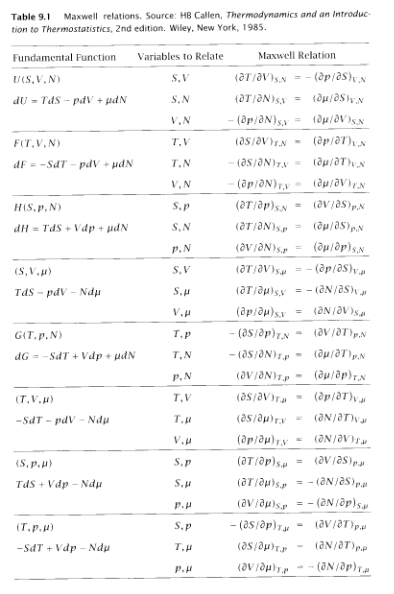
\includegraphics[scale=0.3]{maxrel.png}
  \end{figure}
}

\frame{\frametitle{Tira de borracha}
A energia de uma tira de borracha  dada por:

$$dU=TdS-pdV+fdl$$
 Queremos realizar experimentos com $T$ e $p$ constantes. 
Vamos utilizar portanto $G(p,T,l)$. Temos que:
$$dG=d(H-TS)=d(U+pV-TS)=-SdT+Vdp+fdl$$
Usando estas relaes temos que
$$f=\left( \frac{\partial G}{\partial l}\right)_{T,p}=
    \left( \frac{\partial H}{\partial l}\right)_{T,p}-
   T\left( \frac{\partial S}{\partial l}\right)_{T,p}$$
Podemos obter uma relao de Maxwell para
$$\left( \frac{\partial S}{\partial l}\right)_{T,p}=-
  \left( \frac{\partial f}{\partial T}\right)_{l,p}$$

}


\frame{\frametitle{Tira de borracha}
Temos tambm que:
$$\left( \frac{\partial H}{\partial l}\right)_{T,p}=
f-   T\left( \frac{\partial f}{\partial T}\right)_{l,p}$$
Estas quantidades podem ser medidas experimental medindo como a fora
depende com $T$ para $p$ fixo. 

\begin{center}
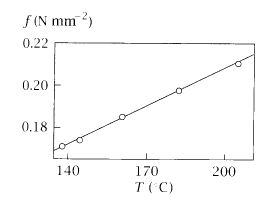
\includegraphics[scale=0.6]{fxT}  
\end{center}

}

\frame{\frametitle{Tira de Borracha}
Note que:
$$\left( \frac{\partial S}{\partial l}\right)_{T,p}=-
  \left( \frac{\partial f}{\partial T}\right)_{l,p}$$
implica pelo grfico que:
$$\left( \frac{\partial S}{\partial l}\right)_{T,p}<0$$

Esta propriedade distingue a borracha dos metais. Isto ocorre por que quanto menor
o comprimento mais liberdade possui o polimero. 


}
\section{Medindo Expanso e Contrao}

\frame{\frametitle{Expanso Trmica}
$$\alpha=\frac{1}{V}\left( \frac{\partial V}{\partial T}\right)_{p}$$
\begin{center}
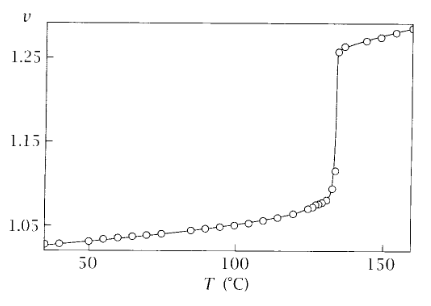
\includegraphics[scale=0.5]{alphaxT}  
Expano do Polietileno
\end{center}
}

\frame{\frametitle{Expanso Trmica}

Exemplo:
Gs Ideal:
$$\alpha=\frac{1}{T}$$


\begin{figure}
\begin{center}
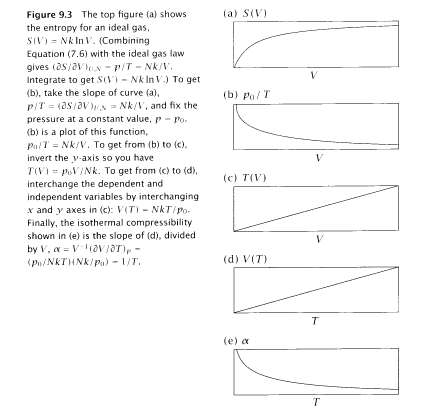
\includegraphics[scale=0.4]{alpha}  
\end{center}
 Expanso trmica e compressibilidade isotrmica 
para a gua e outras lquidos orgnicos (benzeno, n-pantano ter-dietlico)
 
\end{figure}

}


\frame{\frametitle{Compressibilidade Isotrmica}

$$\kappa=-\frac{1}{V}\left( \frac{\partial V}{\partial p}\right)_{T}$$

\begin{center}
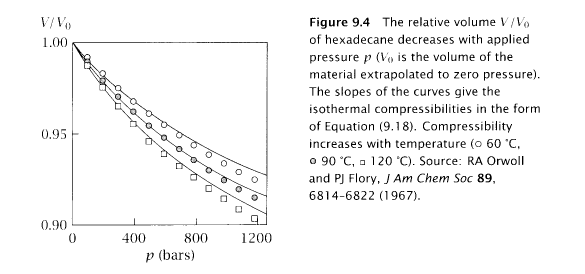
\includegraphics[scale=0.6]{Vxp}  
\end{center}


}

\frame{\frametitle{Expanso Trmica}

Exemplo:
Gs Ideal:
$$\alpha=\frac{1}{p}$$



}
 \frame{\frametitle{gua}
 \begin{tabular}{c c}
     \begin{minipage}{0.45\textwidth}
       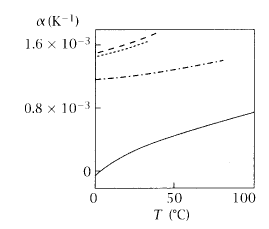
\includegraphics[scale=0.4]{water1}

Coeficiente de expanso trmica para gua (linha cheia) 
e outros lquidos orgnicos
     \end{minipage}&
     \begin{minipage}{0.45\textwidth}
       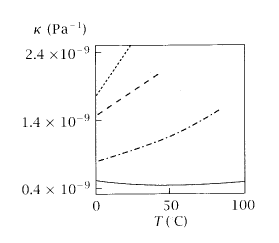
\includegraphics[scale=0.4]{water2}

Compressibilidade para gua (linha cheia) e outros lquidos orgnicos. 
     \end{minipage}
   \end{tabular}
 }



\frame{\frametitle{Mudana de Entropia com a presso}
Considere a dependncia da entropia com a presso:
$$dS=\left( \frac{\partial S}{\partial p}\right)_{T,N}dp
    =-\left( \frac{\partial V}{\partial T}\right)_{p,N}=-\alpha V dp$$
$$\Delta S=\int -\alpha V(p)dp$$
}

\frame{\frametitle{Mudana de Energia com o volume}
Considere a dependncia da energia com o volume:
$$dU=\left( \frac{\partial U}{\partial V}\right)_{T}dV
    +\left( \frac{\partial U}{\partial T}\right)_{V}dT$$

$$dS=\left( \frac{\partial S}{\partial V}\right)_{T}dV
    +\left( \frac{\partial S}{\partial T}\right)_{V}dT$$

Usando estas relaes e a relao fundamental:
$$dU=T\left[ \left( \frac{\partial S}{\partial V}\right)_{T}dV
    +\left( \frac{\partial S}{\partial T}\right)_{V}dT\right]-pdV
$$
}

\frame{\frametitle{Mudana de Energia com o volume}
$$dU=T\left[ \left( \frac{\partial S}{\partial V}\right)_{T}dV
    +\left( \frac{\partial S}{\partial T}\right)_{V}dT\right]-pdV
$$

Se $T=cte$
 $$ \left( \frac{\partial U}{\partial V}\right)_{T}= T \left( \frac{\partial S}{\partial V}\right)_{T}-p$$
Finalmente usando a relao de Maxwell:
$$ \left( \frac{\partial U}{\partial V}\right)_{T}= T \left( \frac{\partial p}{\partial T}\right)_{T}-p$$

}

\section{Sistemas Multicomponentes}
\frame{\frametitle{Volumes Molares Parciais}

Considere um sistema que possua $M$ diferentes espcies qumicas
cada uma caracterizada pelo seu nmero de molculas ou pelo nmero 
de moles:

$${\mathbf n}=n_1, \ldots n_M$$

Para caracterizar estes sistemas usamos Volumes Molares Parciais:

$$v_j=\left( \frac{\partial V}{\partial n_j}\right)_{T,p,n_{i\neq j}}$$

$$dV=\sum_{j=1}^M \left( \frac{\partial V}{\partial n_j}\right)_{T,p,n_{i\neq j}}dn_j=\sum_{j=1}^M v_j dn_j$$


}

\frame{\frametitle{Exemplo lcool}
Eletrostrico

$$V_{app}=\frac{V-n_w v_w}{n_a}$$
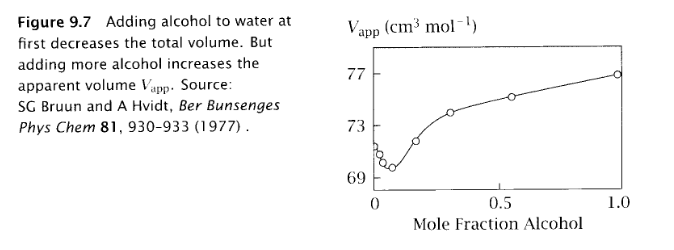
\includegraphics[scale=0.4]{volumemolar}
}

\frame{\frametitle{Exemplo Areia}


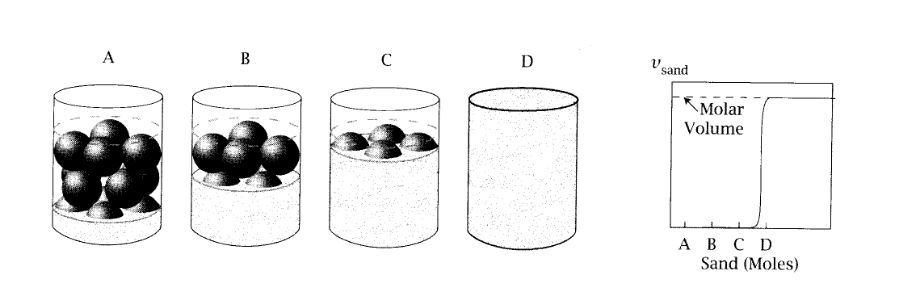
\includegraphics[scale=0.4]{areia}
}


\frame{\frametitle{Potenciais Qumicos}
Como temos que:

$$dU=Tds - pdV +\sum_{j=1}^M\mu_jdN_j$$
$$dH=Tds + Vdp +\sum_{j=1}^M\mu_jdN_j$$
$$dF=-SdT -pdV +\sum_{j=1}^M\mu_jdN_j$$
$$dG=-Sdt + Vdp +\sum_{j=1}^M\mu_jdN_j$$

}

\frame{\frametitle{Potenciais Qumicos}
Podemos definir os potenciais qumicos de vrias formas:

$$\mu_j=\left( \frac{\partial U}{\partial N_j}\right)_{V,S,N_{i\neq j}}
       =\left( \frac{\partial G}{\partial N_j}\right)_{T,p,N_{i\neq j}}
       =\left( \frac{\partial F}{\partial N_j}\right)_{T,V,N_{i\neq j}}
       = \left( \frac{\partial H}{\partial N_j}\right)_{S,p,N_{i\neq j}}
$$
}

\frame{\frametitle{Potenciais Qumicos}
Como os potenciais Qumicos so medidos em condies com presso 
e temperatura fixas, a quantidade de fato mais relevante 
$$\mu_j =\left( \frac{\partial G}{\partial N_j}\right)_{T,p,N_{i\neq j}}
        =\left( \frac{\partial H}{\partial N_j}\right)_{T,p,N_{i\neq j}}-
        T\left( \frac{\partial S}{\partial N_j}\right)_{T,p,N_{i\neq j}} 
        =h_j-Ts_j$$
}

\frame{\frametitle{Funes Homogneas e Potenciais Qumicos}
$$V(\lambda n_1,\ldots ,\lambda n_M)=\lambda V(n_1,\ldots n_M)$$

Como $V$  uma funo homognea temos 

$$V=\sum_{j=1}^M n_j \left( \frac{\partial V}{\partial n_j}\right)_{T,p,n_{i\neq j}}=\sum_{j=1}^M n_jv_j$$

Temos que:

$$dV=\sum_{j=1}^M \left( \frac{\partial V}{\partial n_j}\right)_{T,p,n_{i\neq j}}dn_j=\sum_{j=1}^M v_j dn_j$$


}
\frame{\frametitle{Funes Homogneas e Potenciais Qumicos}
Mas tambm:

$$dV=\sum_{j=1}^M  n_j dv_j+v_j dn_j$$

Logo:

$$\sum_{j=1}^M  n_j dv_j=0$$
}

\frame{\frametitle{Equao de Gibbs-Duhem}
$$U=S\left(\frac{\partial U}{\partial T}\right)_{V,N}d T
   +V\left(\frac{\partial U}{\partial V}\right)_{T,N}d V
   +\sum_{j=1}^M N_j \left(\frac{\partial U}{\partial N}\right)_{V,N_{i,i\neq j}}d N_j
$$

$$U=TS-pV+\sum_{j=1}^M N_j \mu_j$$

Logo temos:

$$dU=TdS+SdT-pdV-Vdp+\sum_{j=1}^M N_j d\mu_j+\sum_{j=1}^M  \mu_j dN_j$$
}

\frame{\frametitle{Equao de Gibbs-Duhem}

Subtraindo esta relao da relao fundamental:

$$\sum_{j=1}^M N_j d\mu_j=Vdp-SdT$$

se $T$ e $p$ so constantes:
$$\sum_{j=1}^M N_j d\mu_j=0$$
}

\frame{\frametitle{Exemplo}
Mostre que em um gs ideal $C_p=C+NK$. 

Um gas ideal satisfaz as equaes:

$$pV=NKT \quad U=U(T)$$ 

$$C_V=\left( \frac{\partial U}{\partial T}\right)_V \quad 
C_p=\left( \frac{\delta q}{\partial T}\right)_p$$

$$C_p=T\left( \frac{\partial S}{\partial T}\right)_p
=\left( \frac{\partial U}{\partial T}\right)_p +
p\left( \frac{\partial V}{\partial T}\right)_p$$
$$C_p=C_V+NK$$

Note que $U$ s depende de $T$ neste caso e portanto a derivada independe tanto 
de $P$ como de $V$. 
}
\end{document}
